\documentclass[11pt]{article}   % Mandatory
\usepackage[T1]{fontenc}        % Support for fonts with æøå and other foreign characters.
\usepackage[utf8]{inputenc}     % Support for UTF-8 encoded input documents
\usepackage{fullpage}
\usepackage{graphicx}           % Support for including graphics as png, gif, and jpeg
\usepackage{amssymb}            % Support for alterantive symbols
\usepackage{amsmath}            % Support for mathematical symbols
\usepackage{listliketab}        % Support for tabulated lists
\usepackage{enumitem}           % Support for indented description items and more
\usepackage[parfill]{parskip}   % Support for American style paragraphs
\usepackage{color}              % Support for colored text
%\usepackage{listings}           % Support for code listings
\usepackage{nameref}            % Enables refernces to names.
\usepackage{makeidx}            % For creating indexes
\usepackage{wasysym}            % For symbols as \smiley
\usepackage{hyperref}        	% For using URLs
\usepackage{xspace}             % For adding a space only when necessary. See ePNS command below.
\newcommand{\epns}{\textbf{Extended Petri net Simulator}\xspace}
\newcommand\writer[1]{\nobreak\begin{flushright}\small\textbf{Author: \large\textit{#1}}\end{flushright}}
\makeindex

\def\signed #1{{\leavevmode\unskip\nobreak\hfil\penalty50\hskip2em
  \hbox{}\nobreak\hfil(#1)%
  \parfillskip=0pt \finalhyphendemerits=0 \endgraf}}

\newsavebox\mybox
\newenvironment{aquote}[1]
  {\savebox\mybox{#1}\begin{quotation}}
  {\signed{\usebox\mybox}\end{quotation}}

\title{UML Diagrams\\ \epns}
\author{Group A}
\date{\today}

\begin{document}
\maketitle

\begin{abstract}
This paper contains the UML diagrams for the major components of the Software Engineering 2 project, which it is a Petri net 3D Simulator. More details about the project can be found in the Project Definition document.
\end{abstract}

\tableofcontents \newpage

\section{Overall model}

Figure \ref{fig:domain-model} presents a high level domain model of the entire system. The user interacts with the system using the editors and the simulator.

\begin{figure}[htp]
\begin{center}
  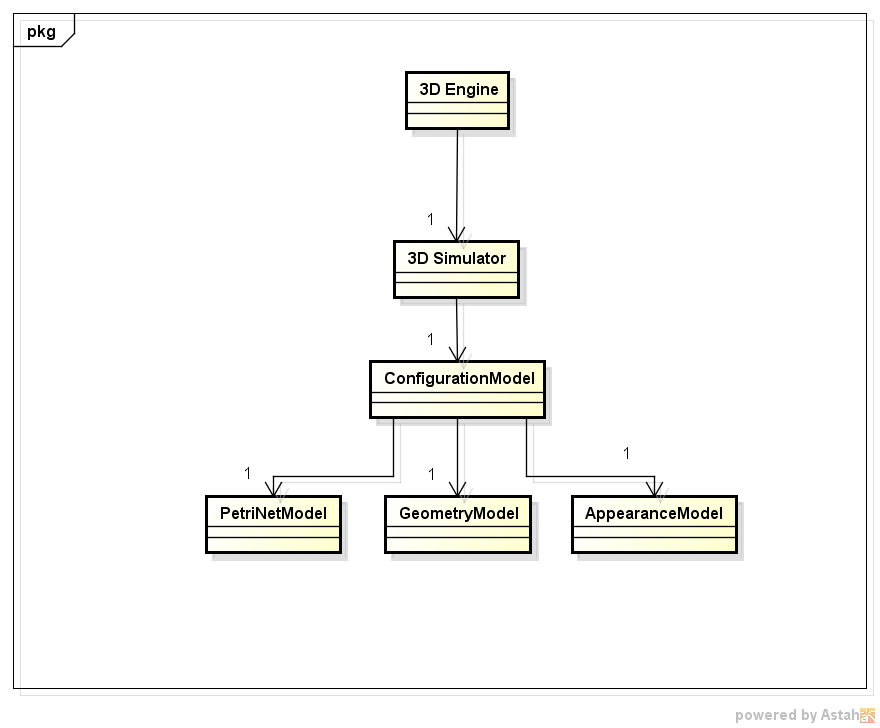
\includegraphics[width=0.8\textwidth]{image/domain_model.png}
  \caption{Domain model}
  \label{fig:domain-model}
\end{center}
\end{figure}

\newpage
\section{Petri net model}

\begin{figure}[htp]
\begin{center}
  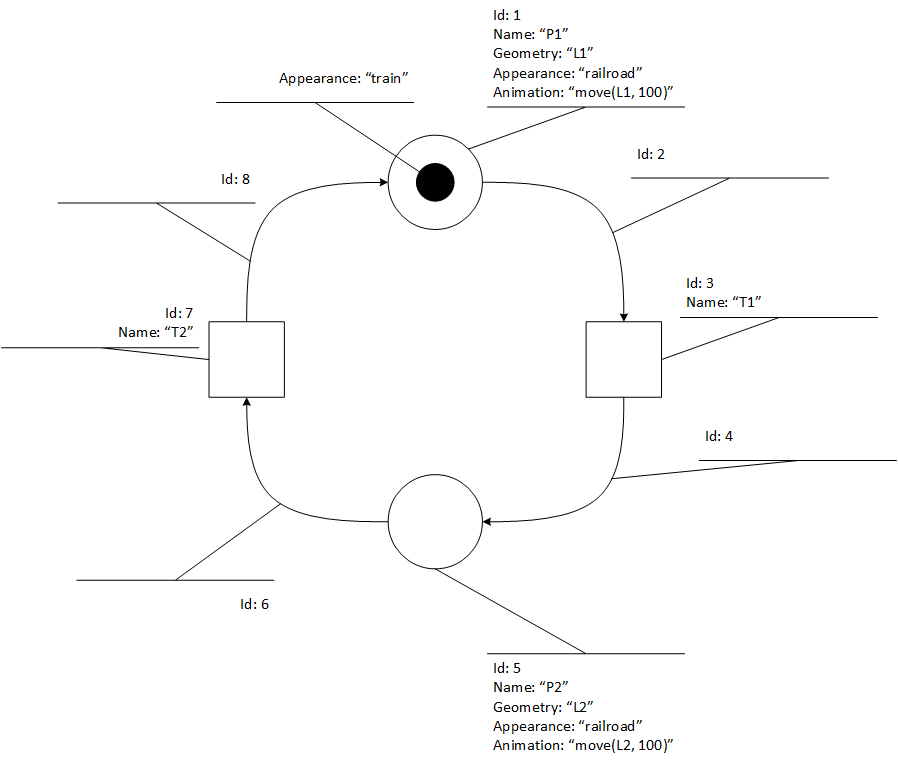
\includegraphics[width=0.6\textwidth]{image/example_petrinet.png}
  \caption{Example of an extended Petri net}
  \label{fig:extended_petrinet}
\end{center}
\end{figure}

Figure \ref{fig:extended_petrinet} shows an example of a particular extended Petri net. On this Petri net, there are two places (P1 and P2), two transitions (T1 and T2), and four arcs that link all the elements. Additionally, places can contain tokens. Moreover, the places contain additional information relevant for the simulator:
\begin{itemize}
\item A geometry label, to link the place to a geometry location
\item An appearance label, to link the place to a specific appearance, with shape, texture,...
\item An input place label, to indicate if the place is a special place that the user can click (for example to change \item the behaviour of the Petri net).
\item An animation label, to indicate how the 3D simulator should animate this place and the tokens contained in it.
\end{itemize}
A token also has an appearance label, in order to define its shape on the simulation.

\begin{figure}[htp]
\begin{center}
  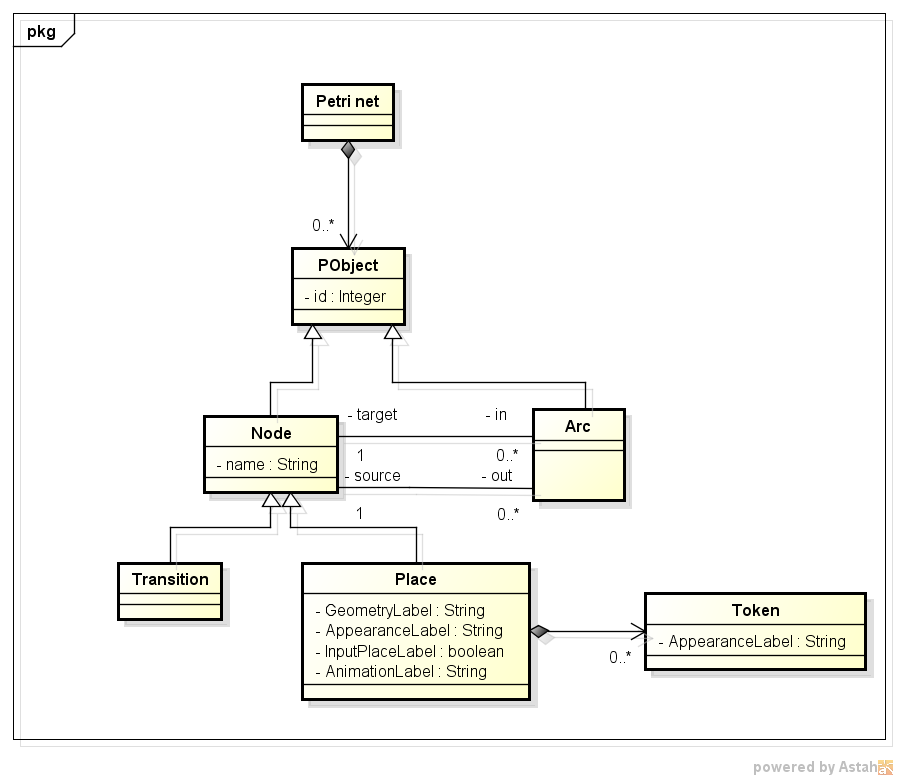
\includegraphics[width=0.8\textwidth]{image/petrinet.png}
  \caption{Petri net model}
  \label{fig:petrinet}
\end{center}
\end{figure}

\section{Geometry model}

\begin{figure}[htp]
\begin{center}
  \includegraphics[width=0.6\textwidth]{image/example_geometry.png}
  \caption{Example of an extended Petri net}
  \label{fig:extended_petrinet}
\end{center}
\end{figure}

\section{Appearance model}

The above diagram describes the domain model associated to the Appearance Editor described in the Project Definition. 
Each appearance model will have one or more objects of type AObject, each corresponding to an element in the Petri Net. The name attribute of each appearance object should be the same as the AppearanceLabel of its corresponding Petri Net object. Moreover, an appearance object has an associated 3DObject which is a file previously defined by the user and loaded in the Appearance Editor. Such a file can contain all or some of the following elements: 
\begin{itemize}
\item shape: sphere, cube, etc.
\item texture
\item color: red, green, black, etc.
\end{itemize}

The Appearance Model will in the end be structured as an XML file which will be used by the Configurator Editor.    

\section{Configuration model}
\section{3D Simulator model}
\printindex



\end{document}

